\section{Introduction}
Two issues of mobile video playback remain unaddressed. Firstly, High Definition (HD) video playback is not supported on many mobile devices due to its heavy processing requirement. Secondly, video playback is energy demanding, which makes the mobile devices unusable quickly. 

The screen on mobile devices is usually not large, despite its high resolution. Zoom and pan gestures have been widely adopted to help users to view photos, maps and web pages. Recent research indicates zoom and pan are helpful for users when watching videos\cite{Khiem:2011:TUU:2072298.2071917}. When a video is scaled up, only part of the video scene is displayed. The visible part is referred as Region-of-Interest (ROI). The simple scale and display approach is inefficient since the entire video scene is decoded but only part of it is displayed. This observation presents an opportunity to achieve more efficient video playback on mobile devices. 

We propose a software approach named selective decoding that improves the efficiency of zoomable video playback. As its name suggests, this approach decodes video selectively based on the ROI captured from user interactions. With the improved efficiency, it is hoped this approach can help to address the two issues mentioned previously.

Our work is based on MPEG4 Part 2 Simple Profile (SP) codec. However this approach should be applicable for other Discrete Cosine Transform (DCT) based video codec. We focus our work on the decoder side of the codec in the local playback context, but the principles and techniques could be extended to encoder and video streaming. A typical MPEG4 SP decoder is illustrated in Fig 1.
 
\begin{figure}
\centering
%\vspace{2.5cm}
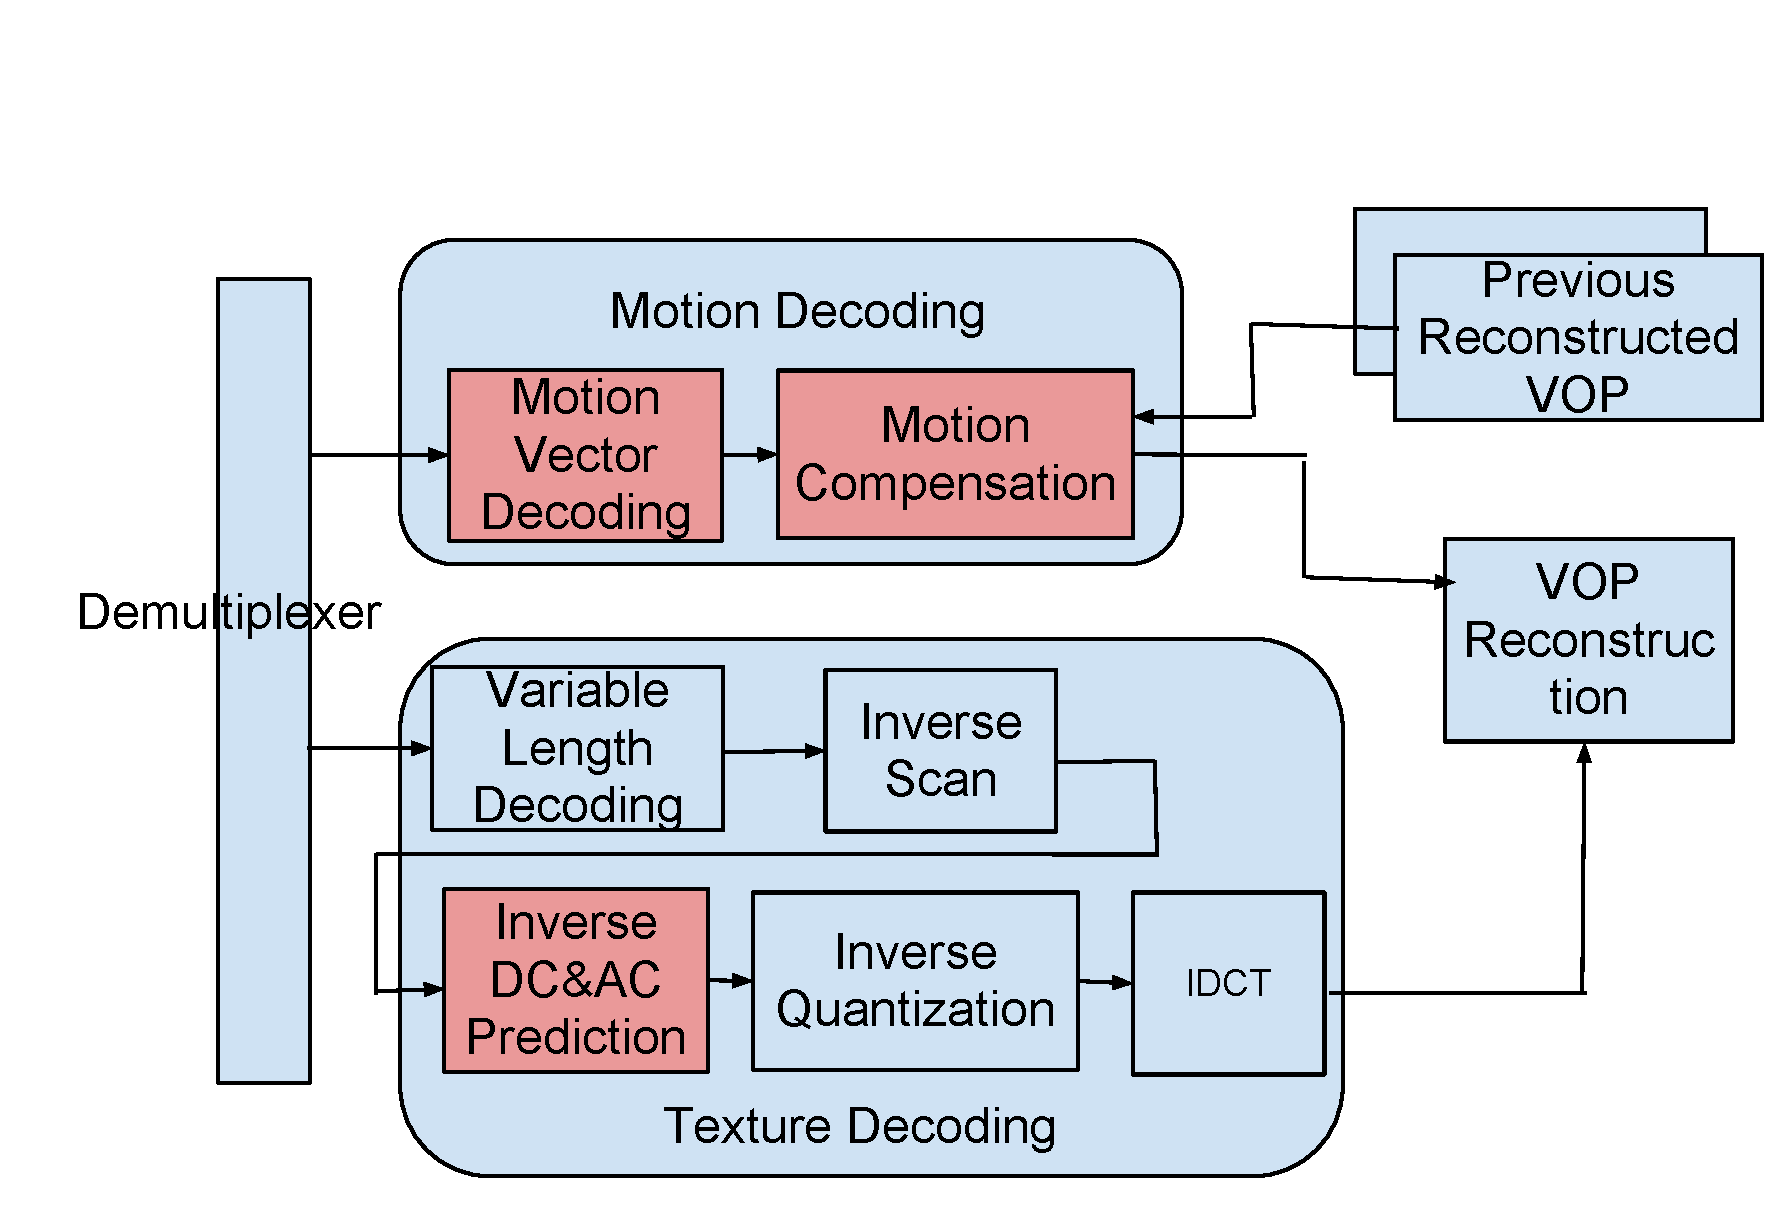
\includegraphics[height=4.3cm]{decoderb.eps}
\caption{A Typical MPEG4 Part 2 Decoder}
\end{figure}
The encoded bitstream is demultiplexed. The coded texture goes through the texture decoding and coded motion is processed by motion decoding. The decoder finally reconstructs the Video Object Plane (VOP). Note that the figure only depicts the core idea of MPEG4 SP decoder, while lots of complexities are not covered. 

Various dependencies exist among macroblocks of a MPEG4 SP coded video. From the decoder's perspective, Inverse DC\&AC Prediction phase at Texture Decoding, and Motion Vector (MV) Decoding and Motion Compensation at Motion Decoding of a macroblock are carried out with reference to other macroblocks. Because of these dependencies, decoding the MBs of a ROI requires macroblocks outside of ROI to be decoded. 

The selective decoding approach pre-processes the video to obtain the dependencies. At decoding, it computes a bitmask based on the dependencies for every frame on the fly, where the selected macroblocks are marked as '1' and others are marked as '0'. The modified decoder then decodes the selected macroblocks accordingly to the bitmask. In this manner, the macroblocks that are necessary and sufficient to present a clear scene at ROI are decoded.

The key contributions in our research are as follows. First, we designed a selective decoding process that decodes user specified ROI efficiently. Secondly, we implemented the selective decoding process as a zoomable video player on Android to demonstrate its practical usage. Finally, we experimentally evaluated the higher frame rate and lower energy consumption benefits of selective decoding over standard decoding. 

In the rest of this paper, Section 2 reviews related works. Section 3 analyzes the dependencies in detail and discusses the offline computation of selective decoding. Online computation is covered in Section 4, including the selective mask generation and modified decoder. The proposed approach is implemented for Android and described in Section 5. We evaluate selective decoding for both playback frame rate and energy consumption in Section 6 and finally conclude at Section 7. 





  


  
